%
% NOIRLab Standard Proposal Attachment
% Draft for Blanco/NEWFIRM HGE target-selection survey
%
\documentclass[11pt]{article}
\usepackage[utf8]{inputenc}
\usepackage{observing-proposal}
\usepackage{xcolor}
\usepackage{epsfig}
\usepackage{graphicx}

% Red text marks quantitative inputs that must be finalized before submission.
\newcommand{\need}[1]{\textcolor{red}{[NEED: #1]}}

\newcommand{\dgr}{$^{\circ}~$}
%\newcommand{\deg}{$^{\circ}$}

\begin{document}

\sciencejustification

{\bf Finding the Metal-Poor Fossil Record of the Inner Milky Way with NEWFIRM}

\noindent\textbf{The hidden metal-poor Milky Way.---}
Metal-poor stars preserve a fossil record of the Milky Way's early assembly,
but our view of that record is strongly biased against the inner disk, bar, and
bulge. Extinction and crowding make these regions inaccessible to most optical
metal-poor-star searches, while conventional near-infrared broad-band colors
cannot cleanly separate metallicity from temperature and reddening. As a
result, metal-poor stars at low Galactic latitude remain among the least
completely mapped populations in the Galaxy. Their distribution and chemical
abundance patterns can distinguish a centrally concentrated remnant of the
proto-Milky Way from early accretion debris and a metal-weak extension of the
disk, directly testing models for the formation of the inner Galaxy.

\smallskip
\noindent\textbf{A photometric solution in the near infrared.---}
We propose a 60~deg$^2$ intermediate-band imaging survey of the inner Galactic
midplane with NEWFIRM on the Blanco 4-m telescope. The NEWFIRM $H1$ and $H2$
filters sample different portions of the $H$-band spectral energy distribution.
Their color changes with metallicity along the upper red-giant branch, while
existing broad-band $J-K_s$ photometry constrains temperature and reddening.
Synthetic photometry shows that this combination separates metal-poor RGB stars
from the much more numerous metal-rich red-clump population that overlaps them
in broad-band color and magnitude (Figure~1). At our expected precision of
$\sigma(H1-H2)\simeq0.011$~mag at $H=15.5$, the predicted displacement is
\need{color separation} and yields \need{completeness} completeness for
$[\mathrm{Fe/H}]<-1$ with \need{purity or contamination reduction} over
\need{RGB color/extinction range}. The proposed observations will test and
empirically calibrate this selection where optical metallicity surveys are
ineffective.

\smallskip
\noindent\textbf{Enabling the Hidden Galaxy Explorer.---}
After-SDSS-V's Hidden Galaxy Explorer (HGE) is being developed to map the
dust-obscured far side of the Milky Way through deep near-infrared spectroscopy
of faint luminous giants. HGE can deliver precise velocities and detailed
abundances, but its scientific return depends on an efficient, well-characterized
input catalog. Existing 2MASS, VIRAC2, UKIDSS-GPS, and GLIMPSE photometry can
identify luminous red giants and estimate extinction through RJCE (Majewski et
al.\ 2011), but cannot efficiently isolate the rare metal-poor population.
Without metallicity preselection, a large fraction of fibers and long integrations would be
spent on metal-rich foreground stars. NEWFIRM supplies the missing metallicity
information. Combining the proposed $H1/H2$ imaging with existing catalogs will
yield \need{number} high-priority candidates to HGE's faint limit of $H=15.5$
across $20^\circ<l<40^\circ$ and $|b|<1.5^\circ$. APOGEE stars in the footprint
will provide an immediate spectroscopic training and validation sample.

\smallskip
\noindent\textbf{Goals and legacy value.---}
The program has three measurable goals: (1) demonstrate and calibrate
intermediate-band selection of $[\mathrm{Fe/H}]<-1$ RGB stars in crowded,
extinguished midplane fields; (2) deliver an HGE target catalog with a
quantified selection function; and (3) constrain the projected density of
metal-poor giants across the surveyed inner-disk sightlines. The calibrated
images and crowded-field photometric catalog will also provide a uniform
near-infrared legacy data set for Galactic structure studies in a region poorly
served by existing surveys.

% Two additional pages may contain references, figures (maximum three), captions.
\clearpage

\begin{figure}[!ht]
\centering
\begin{minipage}[t]{0.32\textwidth}
\centering
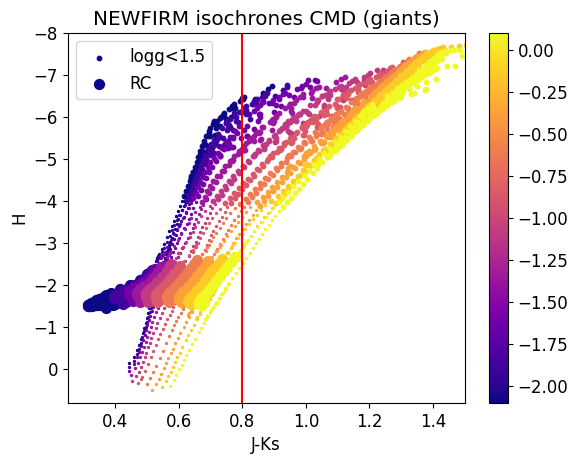
\includegraphics[width=\linewidth]{newfirm_cmd_feh.png}
\textbf{(a)}
\end{minipage}\hfill
\begin{minipage}[t]{0.33\textwidth}
\centering
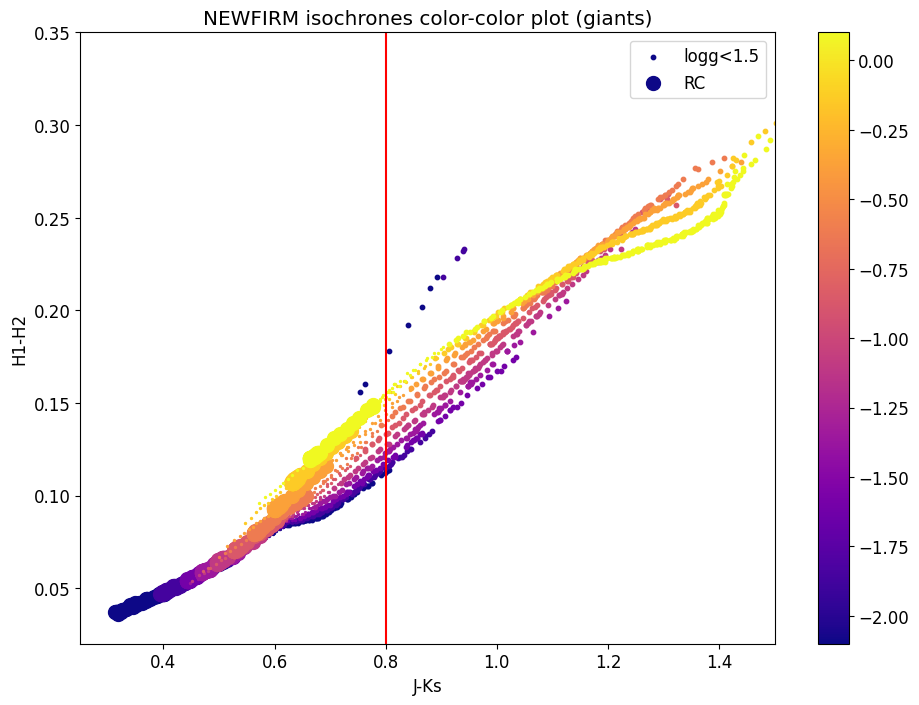
\includegraphics[width=\linewidth]{newfirm_h1-h2_j1-ks_feh.png}
\textbf{(b)}
\end{minipage}\hfill
\begin{minipage}[t]{0.31\textwidth}
\centering
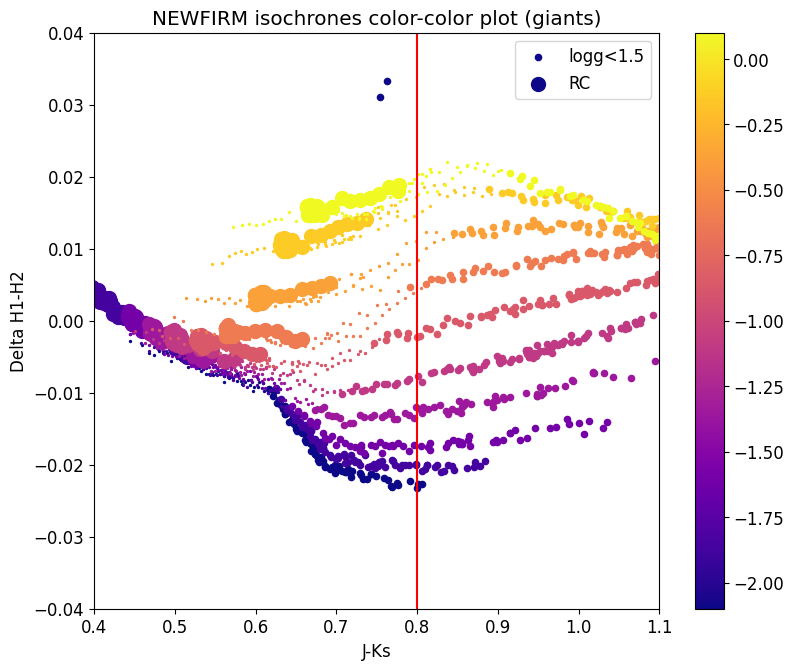
\includegraphics[width=\linewidth]{newfirm_delta_h1-h2_j1-ks_feh.png}
\textbf{(c)}
\end{minipage}
\caption{\textbf{Metallicity sensitivity of the NEWFIRM intermediate bands.}
PARSEC 2.5~Gyr isochrones are shown over a range of metallicities. Red-clump
stars (RC) are marked with large filled circles; smaller filled circles are the
luminous RGB stars ($\log g<1.5$) targeted by HGE.
\textbf{(a)} NEWFIRM color--magnitude diagram for isochrones spanning a range
of metallicity. Metal-rich RC stars overlap the metal-poor
($[\mathrm{Fe/H}]\lesssim-1$) RGB in broad-band color and magnitude.
\textbf{(b)} $H1-H2$ versus $J-K_s$ for the same isochrones; $J-K_s$ traces
temperature while $H1-H2$ provides metallicity leverage.
\textbf{(c)} The same diagram after removing the fitted linear color trend to
highlight the metallicity-dependent displacement. The final selection will use
existing catalog $J-K_s$ photometry, empirically calibrated with APOGEE stars.
%Metallicity-dependent displacement in $H1-H2$ relative to
%\need{define the reference sequence}. \need{Add model family, age, metallicity
%range, extinction treatment, and predicted color separation at the HGE
%magnitude range.}
}
\end{figure}

\begin{figure}[!ht]
\centering
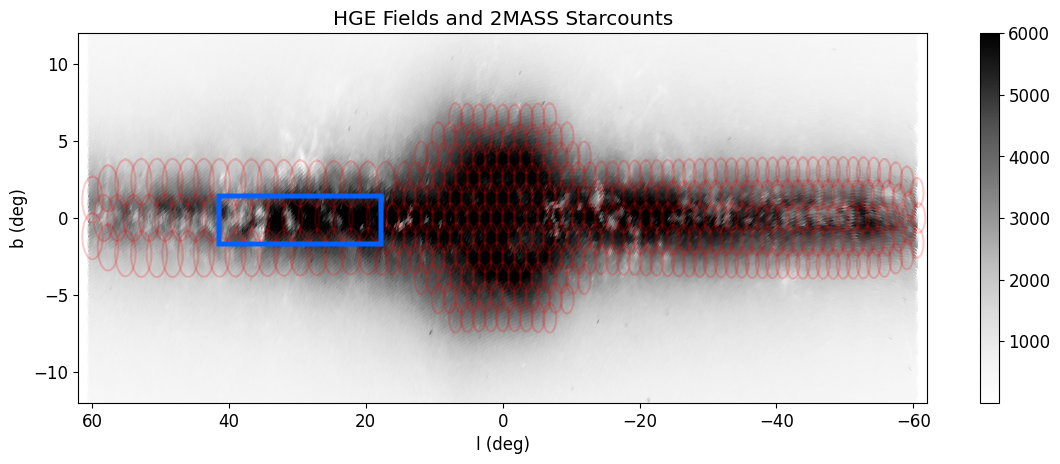
\includegraphics[width=\linewidth]{hge_fields_2mass_starcounts.png}
\caption{\textbf{Proposed survey footprint.}
The proposed 60~deg$^2$ NEWFIRM region (blue) covers
$20^\circ<l<40^\circ$ and $-1.5^\circ<b<1.5^\circ$ within the broader HGE
footprint (red circles), shown over the 2MASS stellar-density map. The HGE test
field at $(l,b)=(340^\circ,+1^\circ)$ is marked in green. The selected region
samples highly extinguished inner-disk sightlines while retaining existing
deep near-infrared coverage and APOGEE stars for calibration.
%\need{Area, longitude/latitude
%limits, number of NEWFIRM pointings, and rationale for field selection.}
}
\end{figure}

\clearpage

\begin{figure}[!ht]
\centering
\fbox{\parbox[c][3.0in][c]{0.92\textwidth}{\centering
PLACEHOLDER---Recovery performance from synthetic or APOGEE-anchored tests:
selection completeness and purity versus magnitude, extinction, or uncertainty.}}
\caption{\textbf{Expected metal-poor target-selection performance.}
\need{Selection boundary and validation data; completeness, purity, and counts.}}
\end{figure}

\begin{references}
\reference Majewski, S.R. et al. 2011, ApJ, 739, 1, 25
\reference APOGEE/HGE reference \need{citation}.
\reference NEWFIRM intermediate-band/NMBS filter reference \need{citation}.
\reference Inner-Galaxy metal-poor-star motivation \need{citations}.
\end{references}

\clearpage

\expdesign

\noindent\textbf{Survey design.---}
We request two May--July nights with Blanco/NEWFIRM to image 60~deg$^2$
of the southern Galactic midplane in the H1 and H2 intermediate bands. The
footprint contains 306 pointings on a $1600\arcsec$ ($26.7\arcmin$) grid,
providing about $1\arcmin$ overlap for astrometric and photometric registration.
At each pointing we will obtain three irregularly offset observations spanning
approximately $60\arcsec$. The three positions partially fill NEWFIRM's
$35\arcsec$ detector gaps, sample each star on independent pixels, and permit
rejection of bad pixels, persistence, and other detector artifacts.

\smallskip
\noindent\textbf{Depth and exposure times.---}
Each observation will contain $2\times10$~s internal coadds, giving 60~s per
filter per pointing. The short coadds keep the H-band background within the
detector's linear regime. For $0.9\arcsec$ image quality, the NEWFIRM exposure
calculator predicts ${\rm S/N}\simeq140$ per band at $H=15.5$, equivalent to
$\sigma(H1-H2)\simeq0.011$~mag before calibration systematics. This precision
is sufficient to measure the metallicity-dependent H1$-$H2 displacement in
Figure~1.

Pointings will be executed in $3\times3$ blocks using the \texttt{DeepSparse}
mapping mode. We will observe all nine pointings in H1, change filters once,
and traverse the grid in reverse in H2. A block covers 1.78~deg$^2$ and is
estimated to require 29 minutes, including readout, dithers, map motions, and
one filter change. The 34 blocks require 16.5 hours of scripted execution;
allowing for acquisition, focus checks, calibrations, and repeated exposures
gives a total requirement of 20 hours, which fits within two long winter
nights.

\smallskip
\noindent\textbf{Conditions and scheduling.---}
We request image quality $\leq1.2\arcsec$ ($\leq1.0\arcsec$ preferred) to
limit blending. Photometric or mostly clear conditions are preferred, but the
dense stellar fields and overlapping tiles provide strong relative
calibration. The program does not require dark time; gray or bright time is
acceptable with a Moon separation of at least $30^\circ$. The fields are
favorably placed during May--July, and the short exposures will be unguided.

\smallskip
\noindent\textbf{Reduction, calibration, and validation.---}
The CTIO NEWFIRM pipeline will perform dark subtraction, flat-fielding, and
bad-pixel correction. For each exposure, a scaled, source-masked sky will be
constructed from the nine nearest same-filter images; every block supplies 27
such images. We will derive astrometry and crowded-field PSF photometry from
the sky-subtracted stacks and use tile overlaps to determine relative
zeropoints. Cross-matches to 2MASS, VIRAC2, APOGLIMPSE, Gaia, and APOGEE will
provide broad-band colors, extinction estimates, and spectroscopic validation.
Artificial-star tests will quantify completeness and color uncertainties. The
final products will be calibrated images, a merged catalog, and an HGE target
list with a quantified selection function.

\end{document}
